% -----------------------------------------------
% Template for ISMIR Papers
% 2015 version, based on previous ISMIR templates
% -----------------------------------------------

\documentclass{article}
\usepackage{ismir,amsmath,cite}
\usepackage{graphicx}
\usepackage{color}
\usepackage{mathrsfs}
\usepackage[english]{babel}
\usepackage{caption}
\usepackage{subfig, color}
\usepackage{microtype}
\sloppy

\usepackage{xspace}
\newcommand*{\eg}{e.g.\@\xspace}
\newcommand*{\ie}{i.e.\@\xspace}

% Title.
% ------
\title{Learning pitch invariants for instrument recognition}


% Single address
% To use with only one author or several with the same address
% ---------------
%\oneauthor
% {Names should be omitted for double-blind reviewing}
% {Affiliations should be omitted for double-blind reviewing}
\oneauthor
{Vincent Lostanlen, Carmine Emanuele Cella, and St\'{e}phane Mallat}
{\'{E}cole normale sup\'{e}rieure}

% Two addresses
% --------------
%\twoauthors
%  {First author} {School \\ Department}
%  {Second author} {Company \\ Address}

% Three addresses
% --------------
%\threeauthors
 %{First author} {Affiliation1 \\ {\tt author1@ismir.edu}}
 %{Second author} {\bf Retain these fake authors in\\\bf submission to preserve the formatting}
 %{Third author} {Affiliation3 \\ {\tt author3@ismir.edu}}

% Four addresses
% --------------
%\fourauthors
%  {First author} {Affiliation1 \\ {\tt author1@ismir.edu}}
%  {Second author}{Affiliation2 \\ {\tt author2@ismir.edu}}
%  {Third author} {Affiliation3 \\ {\tt author3@ismir.edu}}
%  {Fourth author} {Affiliation4 \\ {\tt author4@ismir.edu}}

\begin{document}
%
\maketitle
%
\begin{abstract}
The abstract should be placed at the top left column and should contain about 150-200 words.
\end{abstract}
%

\section{Introduction}\label{sec:introduction}
Among the cognitive attributes of musical tones, pitch is distinguished by a combination of three properties.
First, it is relative: ordering pitches from low to high gives rise to intervals and melodic patterns.
Secondly, it is intensive: multiple pitches heard simultaneously produce a chord, not a single unified tone -- contrary to loudness, which adds up with the number of sources.
Thirdly, it is invariant to instrumentation: this makes possible the transcription of polyphonic music under a single symbolic system. 

Besides this invariance property, understanding the influence of pitch in audio streams is paramount to the design of an efficient system for automated classification, tagging, and similarity retrieval in music. 
Indeed, as demonstrated in the next section, pitch is the major factor of variability among musical notes of a given instrument, if described by existing MIR features.

Time-frequency representations, such as the constant-Q wavelet scalogram, are a useful first step for the construction of pitch-adaptive features.


% audio vs symbolic levels of music information
% variability is dominated by melody and orchestration
% at the symbolic level, melodies are represented over a continuous pitch axis
% whereas instrument identities are categorical and are represented as a histogram
% (that can vary through time)
% music instrument recognition is dual to music transcription

% The problem is made difficult by the fact that factors of variability are entangled.

% Deep convolutional networks have proven to disentangle factors of variability in computer
% vision, such as pose, color, and lighting conditions.


% the challenge is thus two-fold
% 1. gaining abstraction by integrating time-frequency patterns over longer time scales
% 2. building invariants to melody while remaining highly discriminative to the instrument


% On music instrument classification
% Ref to Joder et al
% Ref to Fuhrmann

% On feature learning
% Ref to Dieleman and Benjamin ICASSP 2014
% Ref to Humphrey, Bello, LeCun 2012
% Ref to Salamon and Bello
% Ref to Li, Qian, and Wang arXiv 2015

\section{How invariant is the Mel cepstrum ?}
 
\section{Deep convolutional networks}
\subsection{Time-frequency representation}
We used the implementation from the librosa package \cite{McFee2015} with $Q=12$ filters per octave, center frequencies ranging from 55 Hz to 14 kHz (8 octaves from A1 to A9), and a hop size of 23 ms. Furthermore, we applied nonlinear perceptual weighting of loudness in order to reduce the dynamic range between the fundamental partial and its upper harmonics. A 3-second sound excerpt $\boldsymbol{x}[t]$ is represented by a time-frequency matrix $\boldsymbol{x_1}[t,k_1]$ of width $T=128$ samples and height $K_1=96$ MIDI indices, \ie 8 octaves.

\subsection{Architecture}
First of all, we apply a family $\boldsymbol{W_2}[\tau,\kappa_1,k_2]$ of $K_2=50$ learned time-frequency convolutional operators, whose supports are constrained to have width $\Delta t$ and height $\Delta k_1$. 
\begin{equation}
\boldsymbol{W_2}
\overset{t,k_1}{\ast}
\boldsymbol{x_1}
=
\! \!
\sum_{\substack{
0 \leq \tau < \Delta t \\
0 \leq \kappa_1 < \Delta k_1}}
\! \! \! \! \!
\boldsymbol{W_2}(\tau,\kappa_1,k_2)
\boldsymbol{x_1}[t-\tau,k_1-\kappa_1]
\end{equation}
Furthermore, element-wise biases $\boldsymbol{b_2}[k_2]$ are added to the convolutions, resulting in the tensor 
\begin{equation}
\boldsymbol{y_2}[t,k_1,k_2] =
\boldsymbol{b_2}[k_2] + 
(\boldsymbol{W_2}
\overset{t,k_1}{\ast}
\boldsymbol{x_1})[t,k_1,k_2].
\end{equation}
The second step is the application of a pointwise nonlinearity. We have chosen the \emph{rectified linear unit} [ReLU] because of its popularity in computer vision and its computational efficiency.
 \begin{equation}
 \boldsymbol{y_{2}^{+}}[t,k_1,k_2] = \max \left( \boldsymbol{y_2}[t,k_1,k_2], 0\right)
 \end{equation}
 To achieve invariance to translation as well as frequency transposition, we pool neighboring units in
 the time-frequency domain $(t, k_1)$ over non-overlapping rectangles of width $\Delta t$ and height $\Delta k_1$.
 \begin{equation}
 \boldsymbol{x_2}[t,k_1,k_2] = \! \!
 \max_{
\substack{
0 \leq \tau < \Delta t \\
0 \leq \kappa_1 < \Delta k_1}
 } \! \!
\left\{
 \boldsymbol{y_{2}^{+}}[t - \tau, k_1 - \kappa_1, k_2]
 \right\}
 \end{equation}
 We apply a family $\boldsymbol{W_3}[\tau, \kappa_1, k_2, k_3]$ of $K_3$ convolutional operators that perform a linear combination of time-frequency feature maps in $\boldsymbol{x_2}$ along the channel variable $k_2$.
 \begin{eqnarray}
 \boldsymbol{y_3}[t,k_1,k_3] =
 \qquad  \qquad  \qquad  \qquad  \qquad  \qquad  \qquad \nonumber
 \\
 \sum_{k_2}
 \boldsymbol{b_3}[k_2, k_3]
 + \boldsymbol{W_3}[t,k_1,k_3]
 \overset{t,k_1}{\ast}
 \boldsymbol{x_2}[t,k_1,k_2]
 \end{eqnarray}
After nonlinear rectification and max-pooling, the layer $\boldsymbol{y_3}$ turns into a non-negative tensor $\boldsymbol{x_3}[t,k_1,k_3]$.
\begin{equation}
\boldsymbol{y_4}[k_4] =
\sum_{t,k_1,k_3}
\boldsymbol{W_4}[t, k_1, k_3, k_4]
\boldsymbol{x_3}[t, k_1, k_3]
\end{equation}
We apply nonlinear rectification, yielding $\boldsymbol{x_4}[k_4] = \boldsymbol{y_4^{+}}[k_4]$. $\boldsymbol{y_5}[k_5] = \sum_{k_5} \boldsymbol{W_5}[k_4,k_5] \boldsymbol{x_4}[k_4]$.
\begin{equation}
\boldsymbol{x_5}[k_5] =
\dfrac{\exp \boldsymbol{y_5}[k_5]}
{ \Vert \! \exp \boldsymbol{y_5} \Vert_1}
\end{equation}
The above ensures that the coefficients of $\boldsymbol{x_5}$ are non-negative and sum to one, hence can be fit to a probability distribution.
We define the categorical cross-entropy as

\begin{equation}
\mathscr{L}(\boldsymbol{x_5}, \mathcal{I}) =
- \sum_{k_5 \in \mathcal{I}} \log \boldsymbol{x_5}[k_5].
\end{equation}

The goal is to minimize the average loss $\mathscr{L}(\boldsymbol{x_5}, \mathcal{I})$ for across all pairs $(\boldsymbol{x_5}, \mathcal{I})$ in the training set.

\subsection{Training}
% Random crops
% Categorical cross-entropy
The network is trained on categorical cross-entropy over shuffled mini-batches of size 512 with uniform class distribution. The learning rate policy for each scalar weight in the network is  \emph{Adam} \cite{Kingma2015}, a state-of-the-art online optimizer for gradient-based learning.

% Adam optimizer
% Shuffled examples with uniform class distribution
% Mini-batch learning
% Dropout

\section{Deep supervision of melodic contour}
\subsection{Disentangling pitch from timbre}
% Source-filter equation
% Ref to LeCun on disentangling factors of variability
% Ref to deeply supervised nets
% Ref to NIPS 2015
% Ref to Mallat 2016

\begin{equation}
\mathscr{L}[\boldsymbol{x_2}, \mathcal{P}] =
- \sum_{(t, k_1)\in\mathcal{P}} 
\log \sigma
\left( \sum_{k_2} \boldsymbol{x_2}[t,k_1,k_2] \right)
\end{equation}

\subsection{Joint supervision}
% Different equation
% Comment extraneous vs joint
% Visualization to compare learned filters


\section{Single-instrument classification}\label{sec:single-instrument}
\subsection{Experimental design}
In order to train the proposed algorithms, we used MedleyDB v1.1. \cite{Bittner2014}, a dataset of 122 multitracks annotated with instrument activations as well as melodic $f_0$ curves when present. We extracted the monophonic stems corresponding to a selection of eight pitched instruments [see Figure \ref{fig:instrument-distribution}]. Stems with leaking instruments in the background were discarded.
The evaluation set consists of 120 recordings of solo music collected by Joder et al. \cite{Joder2009}. We discarded recordings with extended instrumental techniques, since they are under-represented in MedleyDB.

\begin{figure}[t]
    \begin{center}
        \setlength{\unitlength}{1cm}
        \begin{picture}(8,10.5)
        \put(0,0){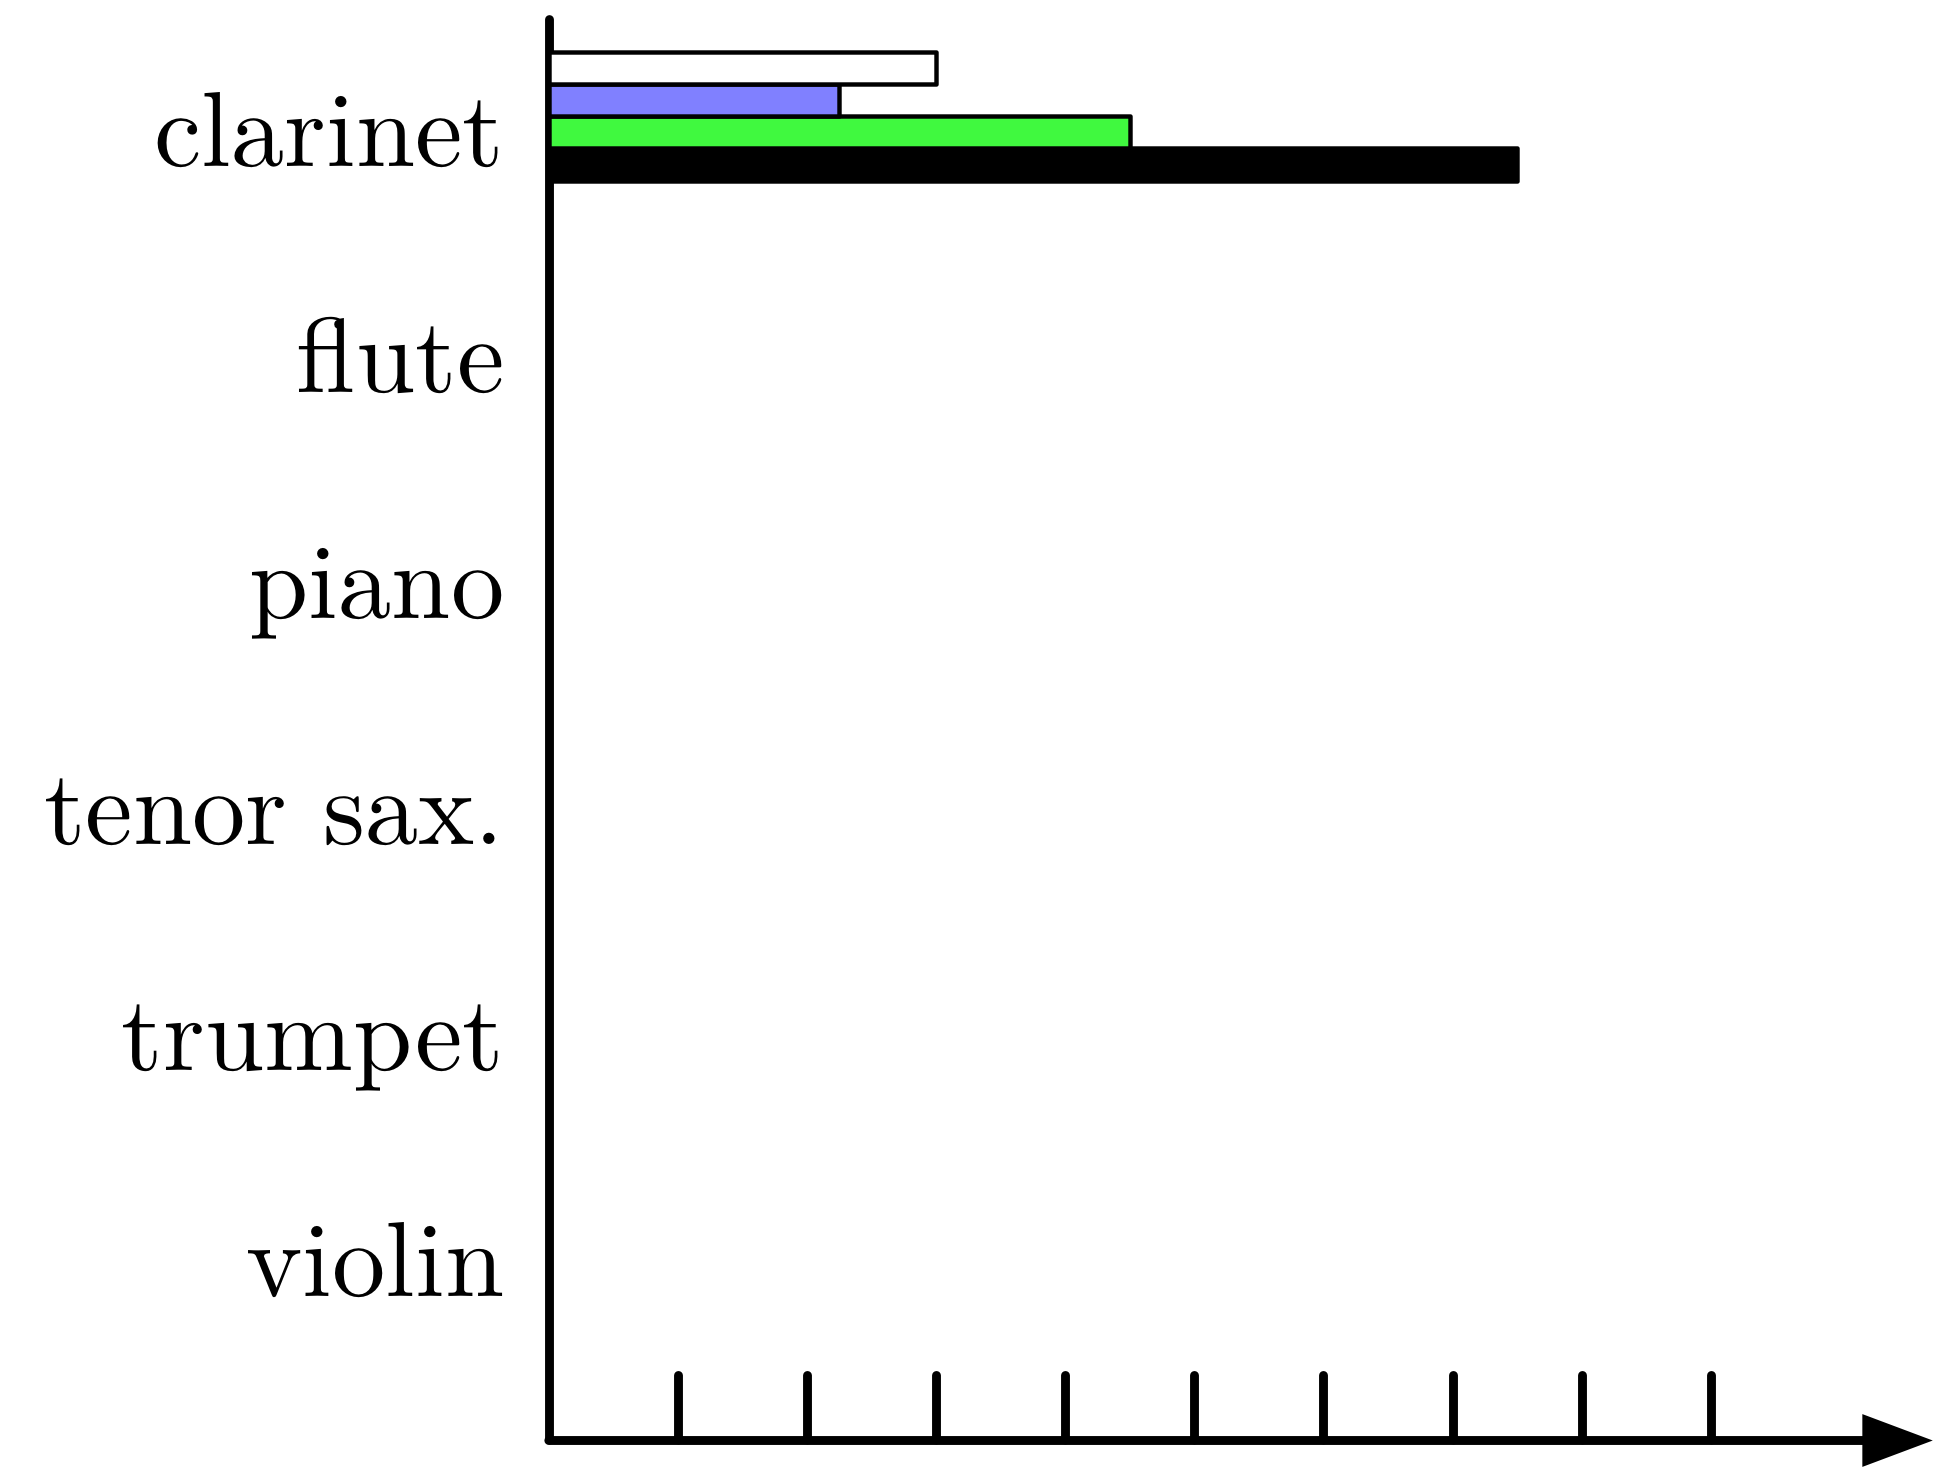
\includegraphics[width=8cm]{figs/mfcc_variances.png}}
        \end{picture}
    \end{center}
    \protect\caption{
    Amount of training data per instrument in MedleyDB, in minutes.
\label{fig:instrument-distribution}
}
\end{figure}

\subsection{Results}


\section{Polyphonic classification}\label{sec:polyphonic}
\subsection{Experimental design}

\subsection{Results}


\section{Conclusions}

% For bibtex users:
\bibliography{ISMIR2015template}

\end{document}
